

\section{Atmospheric Neutrino Post-Fit Correlations}
\label{sec:postfit}


%\begin{figure}[h]
%  \begin{center}
%    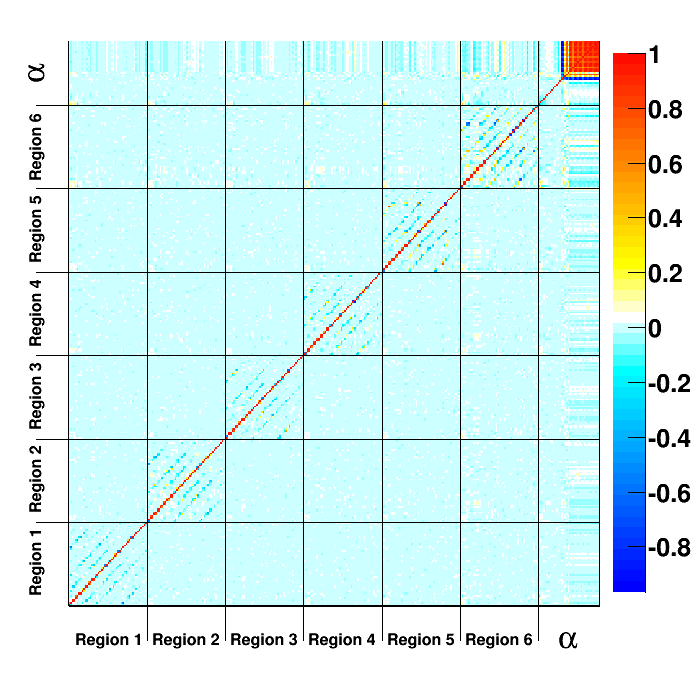
\includegraphics[width=0.7\textwidth]{hcorr_full_labeled}
%  \end{center}
%  \caption{Correlation matrix for all 288 parameters in the atmospheric fit.
%  The labeled regions correspond to the SK detector regions defined in
%  Section~\ref{subsec:DR}.  The region labeled $\alpha$ contains all of the
%  flux, cross section, and normalization parameters.}
%  \label{fig:fitcorr}
%\end{figure}


\begin{figure}[h]
  \begin{center}
    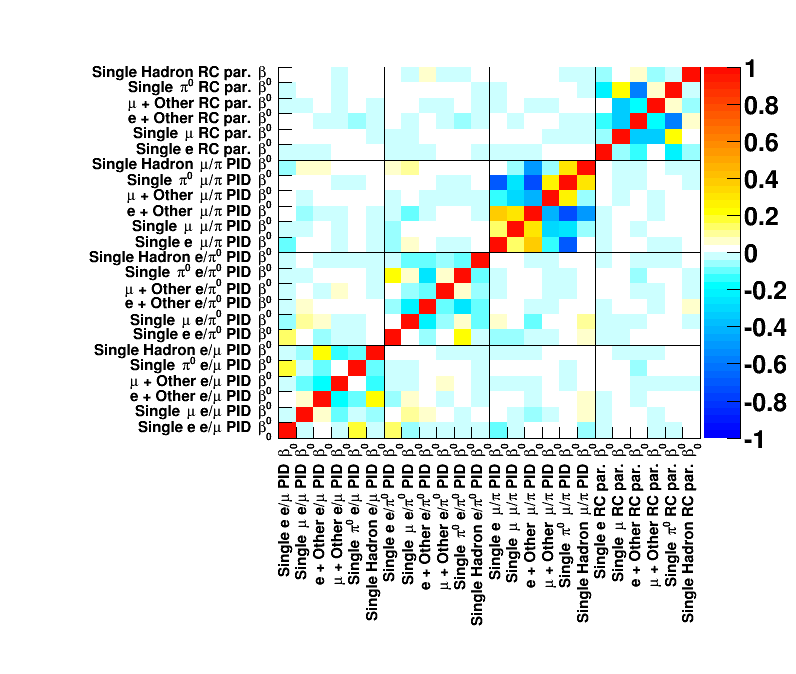
\includegraphics[width=0.85\textwidth]{./cor_beta0.png}
  \end{center}
  \caption{Correlation matrix for all the $\beta^{0}$ parameters (defined in 
  Section~\ref{subsec:betapar}) in detector region 5 (defined in Section~\ref{subsec:DR}).
  Section~\ref{subsec:DR}.}
  \label{fig:fitbeta0corr}
\end{figure}


\begin{figure}[h]
  \begin{center}
    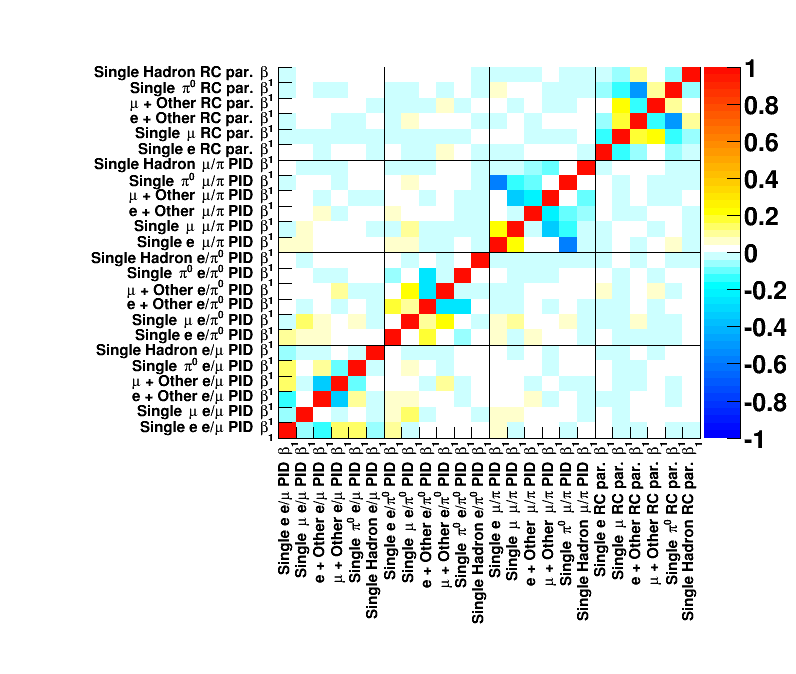
\includegraphics[width=0.85\textwidth]{./cor_beta1.png}
  \end{center}
  \caption{Correlation matrix for all the $\beta^{1}$ parameters (defined in 
  Section~\ref{subsec:betapar}) in detector region 5 (defined in Section~\ref{subsec:DR}).
  Section~\ref{subsec:DR}.}
  \label{fig:fitbeta1corr}
\end{figure}



\begin{figure}[h]
  \begin{center}
    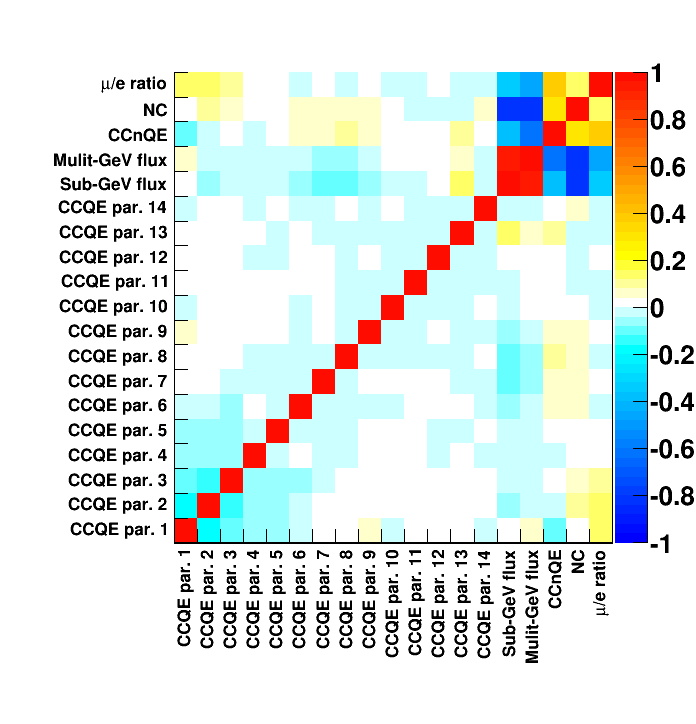
\includegraphics[width=0.85\textwidth]{./cor_alpha0.png}
  \end{center}
  \caption{Correlation matrix for the 19 flux and cross section parameters (defined in 
  Section~\ref{subsec:alphapar}) that affect all of the detector regions.}
  \label{fig:fitalpha0corr}
\end{figure}


\begin{figure}[h]
  \begin{center}
    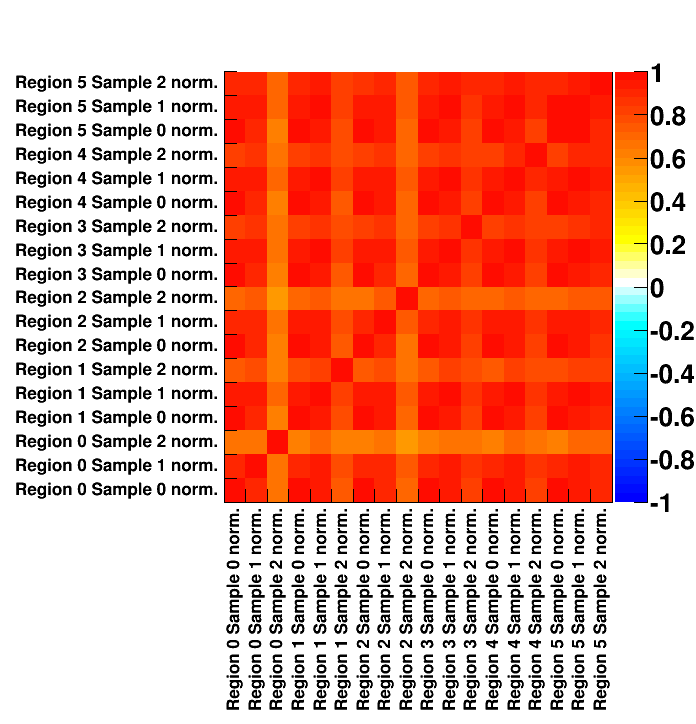
\includegraphics[width=0.85\textwidth]{./cor_alpha1.png}
  \end{center}
  \caption{Correlation matrix for the overall normalization parameters for each
  of the samples defined by the number of decay electrons (the sample numbers
  are defined in Section~\ref{subsec:samples}) in each of the detector regions
  defined in Section~\ref{subsec:DR}.}
  \label{fig:fitalpha1corr}
\end{figure}



